Para el apartado de modelos de clasificación se utilizó un ``\textit{dataset}'' público ({\cite{500images}}), llamado \href{https://www.kaggle.com/datasets/andrewmvd/lung-and-colon-cancer-histopathological-images}{\textit{"Lung and Colon Cancer Histopathological Images"}}, el cual consta de 25,000 imágenes histopatológicas de cáncer de pulmón y de colón. Siendo nuestro interés el cáncer de pulmón, se trabajó únicamente con las imágenes de este tipo de cáncer, las cuales se encuentran divididas en 3 carpetas \textit{"lung\_aca"}, \textit{"lung\_n"} y \textit{"lung\_scc"}, correspondientes a adenocarcinoma, tejido benigno y carcinoma escamocelular respectivamente, cada una de ellas con 5,000 imágenes.

\begin{figure}[h!]
    \centering
    \begin{minipage}{0.3\textwidth} % Ancho de la primera imagen
        \centering
        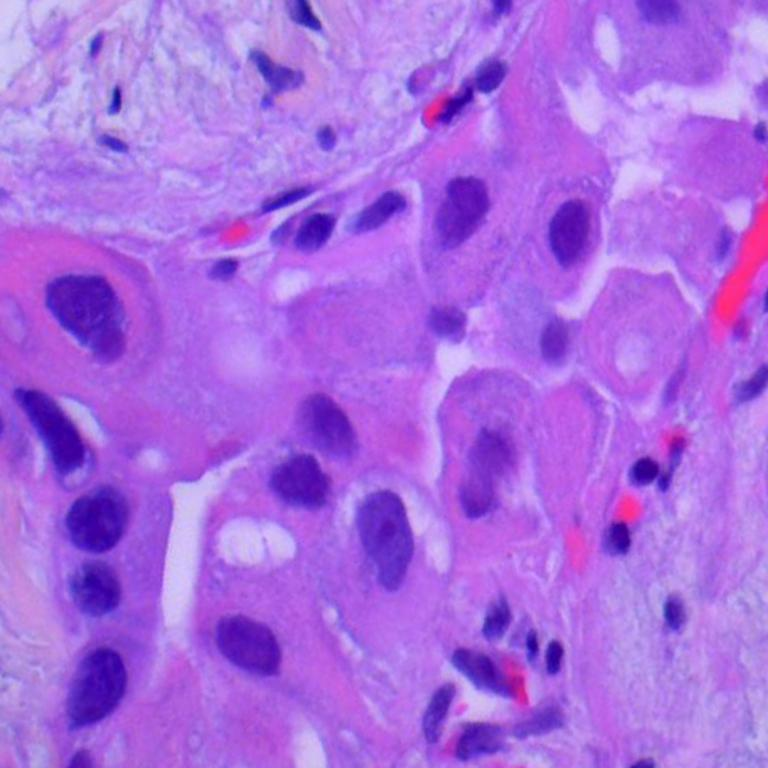
\includegraphics[width=\linewidth]{Francisco/Imagenes metodologia calisficacion/lungaca1.jpeg} % Reemplaza con tu imagen
        \subcaption{Adenocarcinoma} % Subtítulo de la primera imagen
    \end{minipage}
    \hspace{0.5cm} % Espacio entre las imágenes
    \begin{minipage}{0.3\textwidth} % Ancho de la segunda imagen
        \centering
        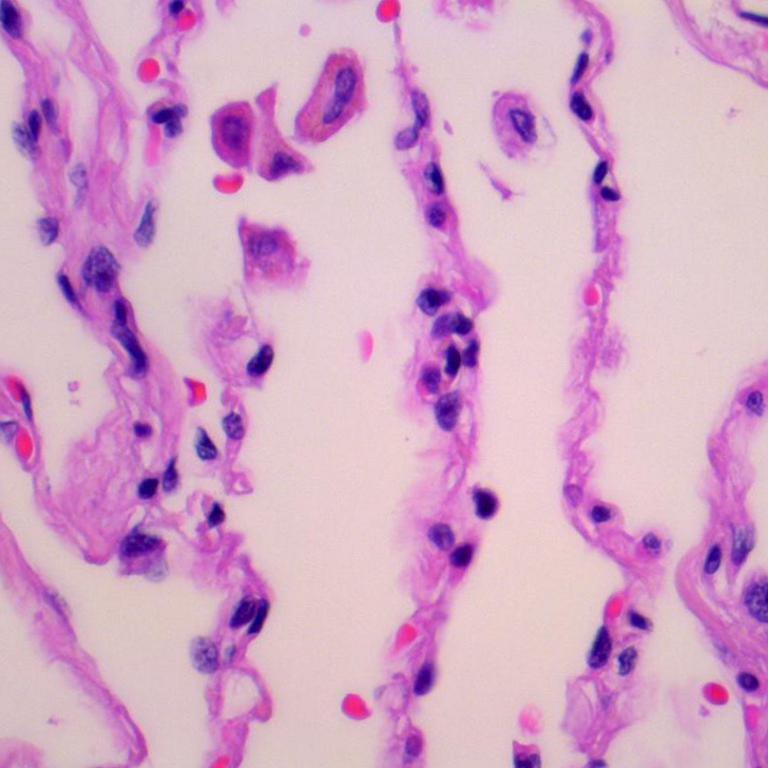
\includegraphics[width=\linewidth]{Francisco/Imagenes metodologia calisficacion/lungn1.jpeg} % Reemplaza con tu imagen
        \subcaption{Benigno} % Subtítulo de la segunda imagen
    \end{minipage}
    \hspace{0.5cm} % Espacio entre las imágenes
    \begin{minipage}{0.3\textwidth} % Ancho de la tercera imagen
        \centering
        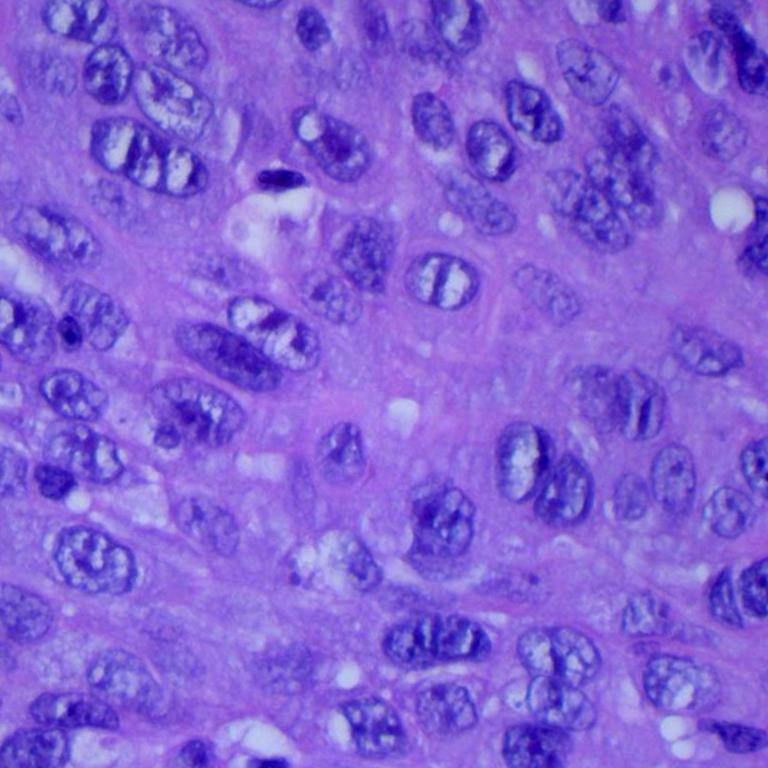
\includegraphics[width=\linewidth]{Francisco/Imagenes metodologia calisficacion/lungscc1.jpeg} % Reemplaza con tu imagen
        \subcaption{Carcinoma} % Subtítulo de la tercera imagen
    \end{minipage}
    
    \caption{Ejemplo de imagen de cada clase}
\end{figure}

Las versiones de \textit{Python}, \textit{pip}, \textit{wheel} y librerías utilizadas, fueron las siguientes:

\begin{itemize}
    \item TensorFlow versión: 2.10.0
    \item NumPy versión: 1.24.4
    \item OpenCV versión: 4.11.0
    \item Matplotlib versión: 3.7.5
    \item Seaborn versión: 0.13.2
    \item Keras versión: 2.10.0
    \item Sklearn versión: 1.3.2
    \item Pip versión: 25.0.1
    \item Python versión: 3.8.0
    \item Wheel versión: 0.45.1
\end{itemize}

Adicionalmente, para los modelos que lo permitían, se utilizó CUDA y cuDNN durante el entrenamiento para acelerar el proceso. Las versiones utilizadas fueron las siguientes:

\begin{itemize}
    \item CUDA versión: 11.8
    \item cuDNN versión: 8.6.0
\end{itemize}

El objetivo en este apartado fue crear modelos que dada una imagen histopatológica de un cáncer de pulmón, pudieran determinar el tipo de tumor entre los 3 mencionados previamente.

Se trabajaron con 2 \textit{"datasets"} diferentes, uno para los modelos existentes en la librería \textit{sklearn}, y otro para los modelos que se crearon con el apoyo de la librería \textit{tensorflow} y \textit{keras}. Esto se debe a que para los modelos creados con \textit{tensorflow} se aprovecharon los métodos y funciones que se encuentran en esta librería, resultando en objetos que podrían causar problemas de compatibilidad o simplemente no se podrían usar con los modelos pertenecientes a la librería \textit{sklearn}. Para el \textit{dataset} utilizado en los modelos de la librería \textit{sklearn} se utilizaron las librerías \textit{cv2} ,\textit{os} y de la librería \textit{sklearn.model\_selection} se importo la clase \textit{train\_test\_split} para la creación de las variables usuales \textit{X\_train}, \textit{X\_test}, \textit{Y\_train} y \textit{Y\_test}, a continuación se muestran los códigos de la definición de estos 2 \textit{datasets} comentados, así como una breve descripción de ambos:\\

\lstset{
    language=Python,
    basicstyle=\ttfamily\footnotesize,
    keywordstyle=\color{blue},
    commentstyle=\color{gray},
    stringstyle=\color{green!60!black},
    numberstyle=\tiny\color{gray},
    numbers=left,
    breaklines=true,
    frame=single,
    captionpos=b,
    tabsize=4,
    showspaces=false,
    showstringspaces=false,
    showtabs=false
}

\begin{lstlisting}[caption={Código creación \textit{dataset} para los modelos de \textit{sklearn}}]
def creacion_dataset(folder):
    
    imagenes = [] # Creacion array de imagenes
    etiquetas = [] # Creacion array de etiquetas
    etiquetas_clases = os.listdir(folder) # Definicion de etiquetas a partir de nombres de carpetas
    
    for etiqueta in etiquetas_clases:
        
        class_path = os.path.join(folder, etiqueta) # Define la ruta de la clase iterada
        if not os.path.isdir(class_path): # Verifica que el folder existe
            continue
        
        for img_name in os.listdir(class_path):
            img_path = os.path.join(class_path, img_name) # Define la ruta de la imagen iterada
            img = cv2.imread(img_path) # Lee la imagen iterada
            if img is not None: # Comprueba que la imagen no es nula 
                img = cv2.resize(img, (64, 64)) # Redimensiona la imagen
                img = cv2.cvtColor(img, cv2.COLOR_BGR2GRAY) # Convierte a escala de grises
                img = img.astype("float32") / 255.0 # "Normaliza" la imagen 
                imagenes.append(img.flatten()) # Convierte el arreglo a una dimension y lo agrega al arrelgo imagenes
                etiquetas.append(etiqueta) # Agrega la etiqueta al arreglo de etiquetas
                
    return np.array(imagenes), np.array(etiquetas) # Retorna los arreglos de imagenes y etiquetas

X, Y = creacion_dataset('Direccion carpetas de imagenes') # Llamado de la funcion

le = LabelEncoder() # Se crea el objeto
Y = le.fit_transform(Y) # Se utiliza el metodo fit_transform para reetiquetar el conjunto de etiquetas

X_train, X_test, Y_train, Y_test = train_test_split(X, Y, test_size=0.2, random_state=42) # Creacion conjuntos de entrenamiento y de test

print(f'Tamano de train: {len(X_train)}, Tamano de test: {len(X_test)}') # Imprime el tamano de los conjuntos de entrenamiento y de test de las imagenes
print(f'Clases codificadas: {le.classes_}')  # Verifica las clases transformadas
\end{lstlisting}

\lstset{
    basicstyle=\ttfamily\footnotesize,    % Mantener la fuente monoespaciada
    backgroundcolor=\color{white},        % Fondo blanco
    keywordstyle=\color{black},           % Palabras clave en negro
    commentstyle=\color{black},           % Comentarios en negro
    stringstyle=\color{black}             % Cadenas en negro
}

\begin{lstlisting}[caption=Salida del código]
Tamano de train: 12000, Tamano de test: 3000
Clases codificadas: ['lung_adenocarcinoma' 'lung_benigno' 'lung_carcinoma']
\end{lstlisting}

Como se dijo previamente esta celda utiliza las librerías \textit{cv2} y \textit{os} para la creación o definición de los conjuntos de entrenamiento y de test. Se utilizó una función que se le da como argumento una cadena con la dirección de la carpeta donde se encuentran las 15,000 imágenes que ya se encuentran separadas en 3 carpetas cada una con 5,000 imágenes con los nombres de las clases. Adicionalmente se importó de la librería \textit{sklearn.preprocessing} la clase \textit{LabelEncoder}, que se utilizó para convertir las etiquetas de tipo \textit{string} a tipo entero, pues algunos modelos no aceptan etiquetas en formato de cadena. \\
Para el preprocesamiento de las imágenes, estas se redimensionaron a un arreglo de 64 x 64, se transformaron a escala de grises pues se buscó evitar un sesgo en el tono de las tinciones entre las diferentes clases. Es decir, se buscó evitar que los modelos simplemente aprendieran a separar entre clases por el tono y no por las características de las imágenes. También se ``normalizaron'' las imágenes dividiendo el valor de cada \textit{pixel} entre 255 para tener únicamente valores entre 0 y 1, y por último se ``aplano'' el arreglo de 2 dimensiones a un arreglo de 1 dimensión.
\\

Para el dataset utilizado en los modelos de \textit{tensorflow} se utilizó el siguiente código para crear los conjuntos de validación y de entrenamiento: \\ 
\\
\\
\\
\\
\lstset{
    language=Python,
    basicstyle=\ttfamily\footnotesize,
    keywordstyle=\color{blue},
    commentstyle=\color{gray},
    stringstyle=\color{green!60!black},
    numberstyle=\tiny\color{gray},
    numbers=left,
    breaklines=true,
    frame=single,
    captionpos=b,
    tabsize=4,
    showspaces=false,
    showstringspaces=false,
    showtabs=false
}

\begin{lstlisting}[caption={Código creación \textit{dataset} para los modelos de \textit{tensorflow}}]
# Definicion de parametros
dataset_dir = "Direccion carpetas de imagenes" # Define la direccion de la carpeta de imagenes
batch_size = 32 # Define el tamano de batch
img_size = (224, 224)  # Ajusta a las dimensiones deseadas
validation_split = 0.2  # Define el tamano del conjunto de validacion
seed = 123  # Fijamos una semilla de aleatoriedad

# Carga del dataset para entrenamiento
train_ds = tf.keras.preprocessing.image_dataset_from_directory(
    dataset_dir,
    validation_split = validation_split,
    subset = "training",
    seed = seed,
    image_size = img_size,
    batch_size = batch_size,
    label_mode = "categorical", # Definimos las etiquetas como categoricas
    shuffle = True # Barajea los registros
)

# Carga del dataset para validacion
val_ds = tf.keras.preprocessing.image_dataset_from_directory(
    dataset_dir,
    validation_split = validation_split,
    subset = "validation",
    seed = seed,
    image_size = img_size,
    batch_size = batch_size,
    label_mode = 'categorical', # Definimos las etiquetas como categoricas
    shuffle = True # Barajea los registros
)

# Verificar etiquetas asignadas
class_names = train_ds.class_names  # Deberia mostrar ['lung_adenocarcinoma', 'lung_benigno', 'lung_carcinoma']
print("Clases asignadas:", class_names)

# Verificar tamanos de los datasets
train_size = tf.data.experimental.cardinality(train_ds).numpy()
val_size = tf.data.experimental.cardinality(val_ds).numpy()

print(f"Entrenamiento: {train_size} batches")
print(f"Validacion: {val_size} batches")

# Funcion para preprocesar las imagenes
def normalize_img(image, label):
    image = tf.image.rgb_to_grayscale(image) # Convierte a escala de grises
    # image = tf.image.grayscale_to_rgb(image) # Esta linea se comenta o no segun la red
    image = tf.cast(image, tf.float32) / 255.0 # "Normaliza" las imagenes
    return image, label

# Aplicar el preprocesamiento a los datasets
train_ds = train_ds.map(normalize_img)
val_ds = val_ds.map(normalize_img)
\end{lstlisting}

\lstset{
    basicstyle=\ttfamily\footnotesize,    % Mantener la fuente monoespaciada
    backgroundcolor=\color{white},        % Fondo blanco
    keywordstyle=\color{black},           % Palabras clave en negro
    commentstyle=\color{black},           % Comentarios en negro
    stringstyle=\color{black}             % Cadenas en negro
}

\begin{lstlisting}[caption=Salida del código]
Found 15000 files belonging to 3 classes.
Using 12000 files for training.
Found 15000 files belonging to 3 classes.
Using 3000 files for validation.
TClases asignadas: ['lung_adenocarcinoma', 'lung_benigno', 'lung_carcinoma']
Entrenamiento: 375 batches
Validacion: 94 batches
\end{lstlisting}

Para la creación de los datasets de entrenamiento y de validación para los modelos creados con \textit{tensorflow}, se utilizó únicamente la clase \textit{image} de la librería \textit{tensorflow.keras.preprocessing}. Al inicio del código se declarán los parámetros a utilizar para evitar reescribirlos, se declara la dirección de la carpeta que contiene las 3 carpetas con las 15,000 imágenes. 


Se declara el tamaño de batch que se utilizará en el entrenamiento, esto es importante pues ya se podra redefinir el tamaño de batch al momento de entrenar los modelos pues esto podría crear incongruencias. \\
Se declara el tamaño de imagen con el que deseamos trabajar y también la semilla de aleatoriedad para poder replicar los resultados. Cabe destacar que el tamaño de la imagen se conservo tan grande pues estos modelos fueron entrenados con el apoyo de \textit{CUDA} por lo que se pudo trabajar con una mayor cantidad de datos. \\
Posteriormente se crean los \textit{datasets} de entrenamiento y de validación utilizando el método \textit{tf.keras.preprocessing.
image\_dataset\_ from\_directory} al cual se le dió los parámetros anteriormente definidos y en adición se definió el parametro\textit{ label\_mode} como ``\textit{categorical}'' pues se trata de una clasificación multiclase y el parámetro \textit{suffle} se declaró como \textit{True} para ``barajear'' las imágenes.\\
Como se puede ver en el código lo que distingue ambos \textit{datasets} no es únicamente el nombre si no también el valor del parámetro \textit{subset}, para el \textit{dataset} de entrenamiento se declara como  \textit{"training"} y para el \textit{dataset} de validación se declara como \textit{"validation"}.\\
Posteriormente se hace una breve comprobación de las clases asignadas así como de la cantidad de \textit{batches} en el conjunto de entrenamiento y en el de validación. \\
Por último se declara una función de preprocesamiento de las imágenes la cual convierte las imágenes a tono de grises y las ``normaliza'' dividiendo cada pixel entre 255 para tener únicamente valores de 0 a 1. Existe una linea en la función que se comenta o no dependiendo del modelo, esto es porque se utilizaron técnicas de \textit{Transfer Learning} y de \textit{Fine Tuning}, por lo que algunos modelos que se usaron de base están diseñados para trabajar con imágenes RGB o de 3 canales. Al transformar las imágenes a escala de grises, reducimos esos 3 canales a 1, provocando una incompatibilidad entre los datos y las dimensiones de entrada de los modelos. Por lo que a veces es necesario ``descomentar'' esta linea para convertir la imagen de vuelta a 3 canales, aunque realmente sigue estando en blanco y negro. \\
Luego de declarada la función se le aplica a los conjuntos por medio del metodo \textit{map} el cual toma como argumento la función a aplicar al objeto que lo llama.

\subsubsection{Support Vector Machine}

Gracias a la disponibilidad de tiempo y de poder computacional disponible del equipo, se tuvo la oportunidad de usar la clase \textit{GridSearchCV} importada de \textit{sklearn.model\_selection} en lugar de la clase \textit{RandomizedSearchCV} para buscar los mejores parámetros de un \textit{Support Vector Classifier} que se encuentra en la librería \textit{sklearn.svm}. A continuación la celda de código comentado, así como su descripción: \\

\lstset{
    language=Python,
    basicstyle=\ttfamily\footnotesize,
    keywordstyle=\color{blue},
    commentstyle=\color{gray},
    stringstyle=\color{green!60!black},
    numberstyle=\tiny\color{gray},
    numbers=left,
    breaklines=true,
    frame=single,
    captionpos=b,
    tabsize=4,
    showspaces=false,
    showstringspaces=false,
    showtabs=false
}

\begin{lstlisting}[caption={Código \textit{GridSearchCV} para \textit{SVC}}]
svm_model = SVC() # Creacion del objeto Support Vector Classifier

# Definicion de parametros a probar
param_grid = {'C': [0.1, 1, 10, 100], 
              "kernel":["linear", "rbf", "poly"],
              'gamma': ['scale', 'auto', 0.01, 0.1, 1, 10, 100]}

# Creacion objeto GridSearchCV con parametros definidos y con 5 CV
grid_search = GridSearchCV(svm_model, param_grid, cv=5, verbose=2, n_jobs=4)
# Entrenamiento de posibles modelos
grid_search.fit(X_train, Y_train)
\end{lstlisting}

Como se explicó, en este código se utilizó la clase \textit{GridSearchCV} por lo que al comienzo se crea un objeto tipo \textit{Support Vector Classifier} para usarlo como parámetro del \textit{GridSearchCV}. Como parámetros adicionales a los ya definidos se declaró \textit{verbose} igual a 2, para poder monitorear constantemente el progreso del modelo y \textit{n\_jobs} igual a 4 para aprovechar los núcleos del procesador sin sobrecalentarlo. Para este modelo se consideraron diferentes valores para \textit{C}, para el \textit{kernel} y para \textit{gamma}, así como 5 \textit{cross-validation's}. Lo que generaba 84 posibles modelos cada uno con 5 \textit{fits} por la validación cruzada, dándonos un total de 420 modelos a entrenar. Esta es una considerable cantidad de modelos de \textit{SVC} y teniéndo en cuenta que suelen tardar en entrenarse por su complejidad, el tiempo estimado de entrenamiento fue alto, pero permisible dados lo recursos del equipo. Por último se aplicó el método \textit{fit} al modelo y se dieron como parámetros los conjuntos creados para los modelos de la librería \textit{sklearn}.

\subsubsection{Regresión Logística}

Al ser un modelo de menor complejidad que un \textit{SVM}, se utilizó nuevamente la clase \textit{GridSearchCV} de la librería \textit{sklearn.model\_selection} y se importó la clase \textit{LogisticRegression} de la librería \textit{sklearn.linear\_model}. A continuación la celda de código comentado, así como su descripción: \\

\begin{lstlisting}[caption={Código \textit{GridSearchCV} para \textit{LogisticRegression}}]
log_reg = LogisticRegression(max_iter=3000) # Creacion del objeto Logistic Regression

# Definicion de parametros a probar
param_grid = {"C": [0.01, 0.1, 1, 10, 100], 
              "penalty": ["l2", "none"], 
              "solver":["liblinear", "lbfgs", "saga"]}

# Creacion objeto GridSearchCV con parametros definidos y con 5 CV
grid_search_lrm = GridSearchCV(log_reg, param_grid, cv=5)
# Entrenamiento de posibles modelos
grid_search_lrm.fit(X_train, Y_train)
\end{lstlisting}

Se creó al comienzo del código un objeto del tipo \textit{LogisticRegression} al cual se le dió como parámetro \textit{max\_iter} el entero 3000, este parámetro determina el número máximo de iteraciones para que el modelo converja, se eligió un número alto de iteraciones ya que los recursos del equipo lo permitían. Adicionalmente a los parámetros a iterar, se declararon 5 \textit{cross-validation's}, para este modelo no se creyó necesario definir los parámetros \textit{n\_jobs} y \textit{verbose} al ser un modelo con poca complejidad. Para este modelo se consideraron diferentes valores de \textit{C}, de \textit{penalty} y de \textit{solver}. Esto generó 30 posibles modelos cada uno con 5 \textit{fits} por la validación cruzada, resultando en un total de 150 modelos a entrenar. Por último se le aplicó el método \textit{fit} al modelo y se dieron como parámetros los conjuntos creados para los modelos de la librería \textit{sklearn}.

\subsubsection{XGBClassifier}

Como último modelo ajeno a \textit{tensorflow} se utilizó la clase \textit{GridSearchCV} para encontrar los mejores parámetros del modelo \textit{XGBClassifier}, el cual se importó de la librería xgboost. Se aprovechó la plataforma de desarrollo CUDA para entrenar este modelo en una GPU, mejorando considerablemente el tiempo de entrenamiento. A continuación la celda de código comentado, así como su descripción: \\

\begin{lstlisting}[caption={Código \textit{GridSearchCV} para \textit{XGBClassifier}}]
modelo_XGB = XGBClassifier(device="cuda", random_state=42)

param_grid = {
    'n_estimators': [100, 200],  # Numero de arboles
    'learning_rate': [0.01, 0.1],  # Tasa de aprendizaje
    'max_depth': [3, 6, 10],  # Profundidad del arbol
    'subsample': [0.7, 1],  # Proporcion de muestras usadas en cada arbol
    'colsample_bytree': [0.7, 1],  # Proporcion de caracteristicas usadas en cada arbol
    'gamma': [0, 0.1],  # Poda del arbol (reduccion de sobreajuste)
    'reg_alpha': [0, 0.1, 1],  # Regularizacion L1
    'reg_lambda': [1, 10, 100],  # Regularizacion L2
    "device": ["cuda"]  # Habilitar GPU
}

# Creacion objeto GridSearchCV con parametros definidos y con 5 CV
grid_search_XGB = GridSearchCV(modelo_XGB, param_grid, cv=5, verbose=2)  
# Entrenamiento de posibles modelos
grid_search_XGB.fit(X_train, Y_train)
\end{lstlisting}

Como en los anteriores modelos, se crea primero un objeto del tipo del modelo que deseamos entrenar, en este caso \textit{XGBClassifier}, para usarlo como parámetro de \textit{GridSearchCV}. Se definió como parámetro de \textit{device}, \textit{cuda}, para aprovechar la GPU disponible del equipo y como \textit{random\_seed} se eligió el entero 42 por si se deseará replicar el modelo. Los parámetros a iterar fueron \textit{n\_estimators} el número de arboles, \textit{learning\_rate} tasa de aprendizaje, \textit{max\_depth} máxima profundidad del árbol, \textit{subsample} cantidad de datos usados, \textit{colsample\_bytree} cantidad de datos usados por árbol, \textit{gamma} poda del árbol, \textit{reg\_alpha} regularización L1, \textit{reg\_lambda} regularización L2 y de manera redundante se volvió a definir el parámetro \textit{device} como \textit{cuda}.

Se creó el objeto GridSearchCV, y se le dió como parámetros el modelo XGBClassifier, los parámetros que se definieron, el parámetro \textit{cross-validation} se definió con el entero 5 y el parámetro \textit{verbose} se definió con 2 para poder monitorear el modelo. Dado la cantidad de parámetros a probar se tienen 864 candidatos, a cada uno se le aplican 5 \textit{fits} por la validación cruzada, siendo el total, 4320 \textit{fits}.

\newpage

\subsubsection{Transfer Learning con MobileNetV2, VGG16 y ResNetRS101}

Se trabajarón 3 modelos usando la técnica de \textit{Transfer Learning}, se usarón como modelo base para cada uno, \textit{MobileNetV2}, \textit{ResNetRS101}, \textit{VGG16}. Se eligió \textit{MobileNetV2} por ser un modelo pequeño y rápido, a pesar de que su uso es en sistemas de visión por computadora en tiempo real. El modelo \textit{VGG16} es un modelo grande, lento y pesado computacionalmente usado para la clasificación de imágenes, por lo que se consideró una buena opción para la problemática presente. Por último se utilizo el modelo \textit{MobileNetV2} el cual es un modelo muy grande y lento pero con una muy alta precisión. Este modelo suele ser utilizado para algunas aplicaciones médicas.

Estos 3 modelos de \textit{Transfer Learning} usaron el \textit{dataset} que se preparo con la librería \textit{tensorflow}. Sus códigos de definición o creación del modelo son prácticamente idénticos excepto por una sola linea de código, a continuación el código comentado de la definición de estas redes y su descripción: \\

\begin{lstlisting}[caption={Código creación CNN con \textit{Transfer Learning} con diferentes modelos base}]
# Se define la variable del modelo base dependiendo cual se usara, sin incluir las capas de salida y con las dimensiones de entrada que se utilizaran

# Modelo base con MobileNetV2
base_model = MobileNetV2(weights="imagenet", include_top = False, input_shape = (224, 224, 3))

# Modelo base con VGG16
base_model = VGG16(weights="imagenet", include_top = False, input_shape = (224, 224, 3))

# Modelo base con ResNetRS101
base_model = ResNetRS101(weights="imagenet", include_top = False, input_shape = (224, 224, 3))


# Se congelan los pesos preentrenados del modelo base
for layer in base_model.layers:
    layer.trainable = False

# Se agregan capas de salida 

# Se agrega una capa de GlobalAveragePooling2D para reducir el numero de parametros
x = layers.GlobalAveragePooling2D()(base_model.output)

# Se agregan dos capas densas de 1024 neuronas con funcion de activacion ReLu
# Se agregan dos capas Dropout para reducir el sobre ajuste
x = layers.Dense(1024, activation='relu')(x)
x = layers.Dropout(0.5)(x)
x = layers.Dense(1024, activation='relu')(x)
x = layers.Dropout(0.5)(x)

# Se agrega una capa densa de 3 neuronas con funcion de activacion softmax como capa de salida
x = layers.Dense(3, activation="softmax")(x)

# Se crea y se compila el modelo usando el modelo base elegido y las capas extras
model = Model(inputs=base_model.input, outputs=x)
model.compile(optimizer=Adam(learning_rate=1e-4), metrics=['accuracy'], loss="categorical_crossentropy")
\end{lstlisting}

Al comienzo del código se definió el modelo base dependiendo cual de los 3 candidatos se usaría, esto comentando y descomentando las 3 diferentes definiciones de la variable \textit{base\_model}. Estos modelos se encuentran alojados en la librería \textit{tensorflow.keras.applications}. Después se cargaron los pesos de \textit{ImageNet} para cualquiera de los 3, no se utilizaron las capas de salida, pues se usaron capas de salidas propias y se definió las dimensiones de los datos de entrada que fueron definidos en la creación de los conjuntos de entrenamiento y de validación. Posteriormente se ``congelaron'' los pesos del modelo base pues se buscó evitar un sobre ajuste y aprovechar los pesos originales del modelo base seleccionado.

Adicionalmente al modelo base elegido, se agregaron capas extras de salida: una capa de \textit{GlobalAveragePooling2D} conectada a la salida del modelo base, en seguida una capa densa, es decir, una capa totalmente conectada, de 1024 neuronas con función de activación ``relu'' para disminuir la complejidad computacional del modelo. Después, una capa de \textit{Dropout} con una probabilidad del 50\% para evitar un sobreajuste y dos capas idénticas a las anteriores para hacer un total de 5 capas. Como capa final se agrego una capa densa de 3 neuronas con función de activación \textit{softmax}, esto debido a que se trata de una clasificación multiclase de 3 clases, de ser una clasificación binaria, se hubiera usado la función de activación sigmoide.

\newpage

Al final del código se definió la variable \textit{modelo} usando la función \textit{Model} a la cual se le dio como parámetros \textit{inputs} y \textit{outputs}, el modelo base seleccionado y las capas de salidas definidas anteriormente. \\
Y por último se utilizó el método \textit{compile} para compilar el modelo usando como parámetros de \textit{optimizer}, \textit{metrics} y \textit{loss}, el optimizador \textit{Adam} con una tasa de aprendizaje de 0.001, la métrica \textit{accuracy} para evaluar el desempeño del modelo en cada época y la función de pérdida \textit{categorical\_crossentropy} pues se trata de un modelo de clasificación multiclase.

Se utilizó el método \textit{summary} para tener una idea del contenido, dimensiones y parámetros de los modelos. Debido a la cantidad de capas y la relevancia para el presente proyecto, se exhibirán únicamente la cantidad de parámetros entrenables, no entrenables y cantidad total de cada uno de estos modelos: \\

\lstset{
    basicstyle=\ttfamily\footnotesize,    % Mantener la fuente monoespaciada
    backgroundcolor=\color{white},        % Fondo blanco
    keywordstyle=\color{black},           % Palabras clave en negro
    commentstyle=\color{black},           % Comentarios en negro
    stringstyle=\color{black}             % Cadenas en negro
}

\begin{lstlisting}[caption={Salida del método summary aplicado a la red de \textit{Transfer Learning} con \textit{MobileNetV2}}]
Total params: 4,622,403
Trainable params: 2,364,419
Non-trainable params: 2,257,984
\end{lstlisting}

\begin{lstlisting}[caption={Salida del método summary aplicado a la red de \textit{Transfer Learning} con \textit{VGG16}}]
Total params: 16,292,675
Trainable params: 1,577,987
Non-trainable params: 14,714,688
\end{lstlisting}

\begin{lstlisting}[caption={Salida del método summary aplicado a la red de \textit{Transfer Learning} con \textit{ResNetRS101}}]
Total params: 64,826,147
Trainable params: 3,150,851
Non-trainable params: 61,675,296
\end{lstlisting}

Posteriormente se procedió al entrenamiento del modelo, este proceso fue exactamente idéntico para los 3 modelos propuestos, a continuación el código comentado y su descripción: \\

\lstset{
    language=Python,
    basicstyle=\ttfamily\footnotesize,
    keywordstyle=\color{blue},
    commentstyle=\color{gray},
    stringstyle=\color{green!60!black},
    numberstyle=\tiny\color{gray},
    numbers=left,
    breaklines=true,
    frame=single,
    captionpos=b,
    tabsize=4,
    showspaces=false,
    showstringspaces=false,
    showtabs=false
}

\begin{lstlisting}[caption={Código entrenamiento de la CNN con \textit{Transfer Learning} sin importar el modelo base}]
# Declaracion parametros EarlyStopping
early_stopping = EarlyStopping(
    monitor='val_loss',       # Monitorea la perdida de validacion
    patience=5,               # Si no mejora en 5 epocas consecutivas, se detiene
    restore_best_weights=True # Restaura los mejores pesos durante el entrenamiento
)

# Se aprovecha CUDA y se entrena con la GPU de la computadora
with tf.device('/GPU:0'):
    history = model.fit(train_ds, 
                        # Se usa el 20% del conjunto de validacion
                        validation_data=val_ds.take(int(tf.data.experimental.cardinality(val_ds).numpy() * 0.2)), 
                        epochs=50, # Se entrena el modelo 50 epocas
                        callbacks=[early_stopping]) # Se define el early stopping
\end{lstlisting}

Esta celda de código tiene como finalidad el entrenamiento del modelo bautizado \textit{model}, el cual puede tener como modelo base cualquiera de los 3 modelos candidatos. Al comienzo se definieron los parámetros del \textit{EarlyStopping}, el cual monitorea la pedida de validación, tiene una paciencia de 5 épocas y se le solicita resturar los pesos con mejor \textit{accuracy} del entrenamiento. Como con modelos anteriores se aprovechó la plataforma de desarrollo \textit{CUDA} como lo refleja el código. Se creó una variable \textit{history} para el entrenamiento con el propósito de poder visualizar el desempeño del modelo a través de las épocas. Utilizando el método \textit{fit} se entrenó el modelo y se le dio como parámetros, el conjunto de entrenamiento, el 20\% del conjunto de validación para evitar un sobreajuste, 50 épocas de entrenamiento y los parámetros del \textit{EarlyStopping}.\\

\newpage

\subsubsection{Fine Tuning con ResNetRS101}

Dados los resultados de los modelos de \textit{Transfer Learning}, los cuales se discutirán más adelante, se decidió usar la técnica de Fine Tuning usando como modelo base únicamente el modelo \textit{ResNetRS101}. A continuación, el código comentado y su descripción: 

\begin{lstlisting}[caption={Código creación CNN con \textit{Fine Tuning} con \textit{ResNetRS101}}]
# Se define la variable base_model usando ResNetRs101, sin incluir las capas de salida y con las dimensiones de entrada que se utilizaran
base_model = ResNetRS101(weights="imagenet", include_top = False, input_shape = (224, 224, 3))

# Se congelan los pesos preentrenados del modelo base
for layer in base_model.layers:
    layer.trainable = False

# Se descongelan las ultimas 20 capas del modelo base
for layer in base_model.layers[-20:]:
    layer.trainable = True

# Se agregan capas de salida

# Se agrega una capa de GlobalAveragePooling2D para reducir el numero de parametros
x = layers.GlobalAveragePooling2D()(base_model.output)

# Se agregan dos capas densas de 1024 neuronas con funcion de activacion ReLu
# Se agregan dos capas Dropout para reducir el sobre ajuste
x = layers.Dense(1024, activation='relu')(x)
x = layers.Dropout(0.5)(x)
x = layers.Dense(1024, activation='relu')(x)
x = layers.Dropout(0.5)(x)

# Se agrega una capa densa de 3 neuronas con funcion de activacion softmax como capa de salida
x = layers.Dense(3, activation="softmax")(x)

# Se crea y se compila el modelo usando el modelo base y las capas extras de salida
model = Model(inputs=base_model.input, outputs=x)
model.compile(optimizer=Adam(learning_rate=1e-4), metrics=['accuracy'], loss="categorical_crossentropy")
\end{lstlisting}

Se definió al comienzo del código la variable \textit{base\_model} usando el modelo base \textit{ResNetRS101} alojado en \textit{tensorflow.keras.applications}. Se cargaron los pesos de ImageNet, no se cargaron las capas de salida y se definieron las dimensiones de los datos de entrada. Eso es idéntico a cuando se utilizó la técnica de \textit{Transfer Learning}.

Como en la técnica de \textit{Transfer Learning} se ``congelaron'' todos los pesos del modelo base para evitar un sobreajuste. Después, para realizar un \textit{Fine Tuning} se ``descongelaron'' las últimas 20 capas del modelo; esto tuvo como objetivo un mayor aprendizaje del modelo.

Posteriormente, exactamente como con los modelos de \textit{Transfer Learning}, se agregaron capas extras de salida: una capa de \textit{GlobalAveragePooling2D} conectada a la salida del modelo base, seguida de una capa densa de 1024 neuronas con función de activación ``relu'', seguida de una capa de \textit{Dropout} con una probabilidad del 50\%, seguidas de una capa densa y una capa \textit{Dropout} idénticas a las primeras. Como capa final del modelo se conectó una capa densa de 3 neuronas con función de activación \textit{softmax} al tratarse de una clasificación multiclase.

Para finalizar, nuevamente como en los modelos de \textit{Transfer Learning}, se creó la variable \textit{model} con la función \textit{Model} a la cual se le dio como parámetros \textit{inputs} y \textit{outputs}, el modelo base y las capas extra respectivamente. Por último, se compiló el modelo con el optimizador \textit{Adam} con una tasa de aprendizaje de 0.0001, como medida de desempeño del modelo la medida \textit{accuracy} y como función de perdida se le dio \textit{categorical\_crossentropy} al tratarse de una clasificación multiclase de 3 clases.

Como con los modelos de \textit{Transfer Learning} se utilizó el método \textit{summary} para tener una idea del tamaño, dimensiones y cantidad de parámetros. Nuevamente, por motivos de cantidad de capas y relevancia para el presente proyecto solo se mostrará la información de los parámetros entrenables, no entrenables y el total de parámetros: \\

\lstset{
    basicstyle=\ttfamily\footnotesize,    % Mantener la fuente monoespaciada
    backgroundcolor=\color{white},        % Fondo blanco
    keywordstyle=\color{black},           % Palabras clave en negro
    commentstyle=\color{black},           % Comentarios en negro
    stringstyle=\color{black}             % Cadenas en negro
}

\begin{lstlisting}[caption={Salida del método summary aplicado a la red de \textit{Fine Tuning} con \textit{ResNetRS101}}]
Total params: 64,826,147
Trainable params: 11,812,867
Non-trainable params: 53,013,280
\end{lstlisting}

El entrenamiento del modelo se hizo de manera idéntica a los anteriores con la siguiente celda de código: \\

\lstset{
    language=Python,
    basicstyle=\ttfamily\footnotesize,
    keywordstyle=\color{blue},
    commentstyle=\color{gray},
    stringstyle=\color{green!60!black},
    numberstyle=\tiny\color{gray},
    numbers=left,
    breaklines=true,
    frame=single,
    captionpos=b,
    tabsize=4,
    showspaces=false,
    showstringspaces=false,
    showtabs=false
}

\begin{lstlisting}[caption={Código entrenamiento de la CNN con \textit{Fine Tuning}}]
# Declaracion parametros EarlyStopping
early_stopping = EarlyStopping(
    monitor='val_loss',       # Monitorea la perdida de validacion
    patience=5,               # Si no mejora en 5 epocas consecutivas, se detiene
    restore_best_weights=True # Restaura los mejores pesos durante el entrenamiento
)

# Se aprovecha CUDA y se entrena con la GPU de la computadora
with tf.device('/GPU:0'):
    history = model.fit(train_ds, 
                        # Se usa el 20% del conjunto de validacion
                        validation_data=val_ds.take(int(tf.data.experimental.cardinality(val_ds).numpy() * 0.2)), 
                        epochs=50, # Se entrena el modelo 50 epocas
                        callbacks=[early_stopping]) # Se define el early stopping
\end{lstlisting}
\subsubsection{Propuesta de CNN}

Como último modelo propuesto en el apartado de clasificación y adicionalmente a los modelos con técnicas de \textit{Transfer Learning} y \textit{Fine Tuning}, se propuso una Red Neuronal Convolucional de diseño propio. A continuación el código de su diseño comentado y su descripción: 

\begin{lstlisting}[caption={Código diseño propio de CNN}]
# Propuesta de CNN

# Se define un modelo secuencial, las capas se agregan una tras la otra
model = models.Sequential([
    
    # Primer conjunto de capas
    # Capa convolucional con 64 filtros de 3x3 con funcion de activacion relu, esta capa es particular porque es la primera, por lo que tambien se definen las dimensiones de entrada
    layers.Conv2D(filters=64, kernel_size=(3,3), activation="relu", input_shape=(224, 224, 1)),
    # Capa MaxPooling2D reduce las dimensiones de la imagen a la mitad
    layers.MaxPooling2D((2,2)),
    
    # Segundo conjunto de capas
    # Capa convolucional de 128 filtros de 3x3 con funcion de activacion relu
    layers.Conv2D(filters=128, kernel_size=(3,3), activation="relu"),
    # Capa MaxPooling2D reduce las dimensiones de la imagen a la mitad
    layers.MaxPooling2D((2,2)),
    
    # Tercer conjunto de capas
    # Capa convolucional de 256 filtros de 3x3 con funcion de activacion relu
    layers.Conv2D(filters=256, kernel_size=(3,3), activation="relu"),
    # Capa MaxPooling2D reduce las dimensiones de la imagen a la mitad
    layers.MaxPooling2D((2,2)),
    
    # Capas de salida
    # Aplana la salida de 2D a un vector de 1D
    layers.Flatten(),
    # Capa densa de 128 neuronas con funcion de activacion relu y una capa dropout con 0.4 de probabilidad
    layers.Dense(128, activation="relu"),
    layers.Dropout(0.4),
    # Capa densa de 64 neuronas con funcion de activacion relu y una capa dropout con 0.4 de probabilidad
    layers.Dense(64, activation="relu"),
    layers.Dropout(0.4),
    # Capa de salida densa con 3 neuronas con funcion de activacion softmax
    layers.Dense(3, activation="softmax")
])

# Compilacion del modelo
model.compile(optimizer=Adam(learning_rate=1e-4), metrics=["accuracy"], loss="categorical_crossentropy")
\end{lstlisting}

El diseño propuesto se trata de una CNN al usar capas convolucionales. Se declaró al inicio del código la variable \textit{model} con ayuda de la función \textit{models.Sequential}. Se le dio como parámetros las diferentes capas que conformarían este modelo, se comenzó con una capa convolucional de 64 filtros de tamaño 3x3 con función de activación \textit{relu}, esta capa tenía la particularidad de ser la capa de entrada por lo que tambien se le dio las dimensiones de entrada de este modelo. Al ser un modelo de diseño propio no fue necesario ``convertir'' los conjuntos de validación y entrenamiento a 3 canales como con los modelos de \textit{Transfer Learning} y \textit{Fine Tuning}, por lo que se conservaron las dimensiones originales de las imágenes, es decir, escala de grises o un solo canal. Seguida a esta capa convolucional se agregó una capa \textit{MaxPooling2D} para reducir las dimensiones de la imagen a la mitad.

El segundo conjunto de capas siguió un diseño similar, teniendo en seguida otra capa convolucional de 128 filtros de dimensiones 3x3 con función de activación \textit{relu} y una capa \textit{MaxPooling2D} para reducir nuevamente las dimensiones de la imagen a la mitad. El tercer conjunto de capas es idéntico al anterior con la única diferencia de que en lugar de 128 filtros, la capa convolucional cuenta con 256 filtros.

El conjunto de capas de salida comienza con una capa \textit{Flatten} que convierte la salida 2D de la última capa convolucional a un vector de 1D para conectar con las capas densas. En seguida, se conectó una capa densa de 128 neuronas con función de activación \textit{relu} y una capa \textit{Dropout} con una probabilidad del 40\% de apagar neuronas para evitar un sobreajuste. Siguiendo a estas dos se conectaron dos capas idénticas con la diferencia de que la capa densa en lugar de tener 128 neuronas tiene 64. Para la última capa, la capa de salida, se conectó una capa densa de 3 neuronas con función de activación \textit{softmax} pues se trata de una clasificación multiclase de 3 clases.

Al final del código, se compila el modelo con el método \textit{compile}. Se le dio como parámetros, \textit{oprtimizer}, \textit{metrics} y \textit{loss}, el optimizador \textit{Adam} con una tasa de aprendizaje de 0.0001, \textit{accuracy} como métrica de desempeño del modelo y la función de pérdida \textit{categorical\_crossentropy} al tratarse de una clasificación multiclase.

Como con todos los modelos anteriores, se volvió a usar el método \textit{summary} en el modelo propuesto. A continuación, la cantidad de parámetros que muestra el método: \\

\lstset{
    basicstyle=\ttfamily\footnotesize,    % Mantener la fuente monoespaciada
    backgroundcolor=\color{white},        % Fondo blanco
    keywordstyle=\color{black},           % Palabras clave en negro
    commentstyle=\color{black},           % Comentarios en negro
    stringstyle=\color{black}             % Cadenas en negro
}

\begin{lstlisting}[caption={Salida del método summary aplicado a la CNN propuesta}]
Total params: 22,529,411
Trainable params: 22,529,411
Non-trainable params: 0
\end{lstlisting}

El entrenamiento fue idéntico al de los otros modelos de redes neuronales, utilizándose exactamente el mismo código que con los anteriores modelos: \\

\lstset{
    language=Python,
    basicstyle=\ttfamily\footnotesize,
    keywordstyle=\color{blue},
    commentstyle=\color{gray},
    stringstyle=\color{green!60!black},
    numberstyle=\tiny\color{gray},
    numbers=left,
    breaklines=true,
    frame=single,
    captionpos=b,
    tabsize=4,
    showspaces=false,
    showstringspaces=false,
    showtabs=false
}

\begin{lstlisting}[caption={Código entrenamiento de la CNN propuesta}]
# Declaracion parametros EarlyStopping
early_stopping = EarlyStopping(
    monitor='val_loss',       # Monitorea la perdida de validacion
    patience=5,               # Si no mejora en 5 epocas consecutivas, se detiene
    restore_best_weights=True # Restaura los mejores pesos durante el entrenamiento
)

# Se aprovecha CUDA y se entrena con la GPU de la computadora
with tf.device('/GPU:0'):
    history = model.fit(train_ds, 
                        # Se usa el 20% del conjunto de validacion
                        validation_data=val_ds.take(int(tf.data.experimental.cardinality(val_ds).numpy() * 0.2)), 
                        epochs=50, # Se entrena el modelo 50 epocas
                        callbacks=[early_stopping]) # Se define el early stopping
\end{lstlisting}